\section{Methodology}

Recent advances in deep learning have drastically improved image classification, especially in domains with fine-grained visual features like textile categorization. The problem of fabric classification can become cumbersome when textile types possess significant similarities (e.g., cotton vs. polyester), fluctuating light conditions, and/or blended compositions. Synthetic measures which mainly characterize a fabric type using Convolutional Neural Networks (CNN) have exhibited decent performance in fabric categorization by capturing some of the local textures and patterns of the fabrics as classifiers \cite{hong2024research, kampouris2016fine}. However, while well-suited for a range of image-based applications, CNNs are often deficient in their ability to capture the long range dependencies context of data sets, which can be critical in discriminating visually similar materials. 

Vision Transformers (ViTs) an advanced model that can model global relationships in image data through self-attention based mechanisms \cite{dosovitskiy2020vit} have shown strong performance in generic image recognition tasks, but only few researchers have recently used it for fabric classification \cite{chitra2023fabric}. 

Driven by the pros and cons of both processes, this work proposes a hybrid deep learning model which includes CNN and ViT processes parallelly. The hybrid model leverages the \textit{local feature extraction capabilities of CNNs} and \textit{global context modeling capabilities of ViTs} to enhance classification accuracy from different textile fabric types. The proposed hybrid architecture of the model is based on the combined work of Chitra et al.~\cite{chitra2023fabric} and Zhong et al.~\cite{hong2024research}, which have shown promising results in fabric classification tasks.

This methodology section explains the architecture associated with this proposed model, the role played by each part of the model, details the proposed feature fusion method, and briefly covers how the final label is produced. The proposed hybrid architecture supports end-to-end training and used rigorously labeled fabric datasets to test the architecture.

\subsection{Convolutional Neural Networks (CNNs)}

Convolutional Neural Networks (CNNs) are now one of the foundations in the computer vision space due to their ability to automatically learn hierarchical feature representations directly from raw image data. While, CNNs have been made famous for their extents in handwritten digit recognition and object detection, CNN architectures also have a striking record of performance in cases where texture, shape, and local pattern are paramount features of among categories - for example, textile type, or fabric categories.

Usually, a CNN consists of a series of convolutional layers and follows these layers with non-linear activation functions (including ReLU), pooling layers, and fully connected layers. The convolutional layers are feature extractors that learn local filters. The filters can learn to detect edges, textures, and patterns at successively higher levels of abstraction. Therefore the deeper you make the network, the more complex and semantically rich representations it builds, which can be applied for correctly classifying fabric-types that exhibit subtle differences in weave, fiber orientation, or surface reflectivity~\cite{simonyan2015vgg, lecun1998gradient}.

In this project, a CNN-based stream is proposed as a hybrid model, consisting of four convolution blocks where the number of output channels doubles after each convolution block (8, 16, 32, 64). Each block represents a 3×3 convolution with a stride of 3 and outputs a tensor with a ReLU activation specification. This architecture efficiently decreases spatial resolution while encoding important texture and pattern information; a method previously demonstrated to be effective for textile classification~\cite{hong2024research}.

Investigations like those carried out by Kampouris et al.~\cite{kampouris2016fine} and Hong et al.~\cite{hong2024research} highlight the effectiveness of CNNs to accomplish fabric type classification based on characteristics including physical, surface and structural properties. Additionally, in a practical setting, CNNs are preferred due to their ability to generalize to real-world textile images with various lighting conditions and camera settings.

Although CNNs can learn features locally quite well, they are fundamentally limited in their ability to capture global dependencies across spatial locations. This may limit CNN performance when more patterned fabrics are encountered. In this research study, CNNs are combined with Vision Transformer (ViT) encoders, elaborated in the next section, to learn local and global representations of fabric structures.

\subsection{Vision Transformers (ViTs)}

Vision transformers (ViTs) have become a strong alternative to convolutional architectures for image classification tasks. ViTs avoid limiting themselves to local receptive fields, as CNNs do, in favor of a patient self-attention approach that allows for modeling of global relations between various parts of an image. This spatial modeling of context is key to a broad number of scenarios including fabric classification where both the spatial layout and contextual relations between textures patterns are relevant to the task~\cite{dosovitskiy2020vit}.

A typical Vision Transformer works by first splitting an image into fixed-size patches (e.g., 16×16 pixels), which are then flattened and linearly projected into a latent embedding space. The patch embeddings, along with the learnable class token and positional embeddings, are then sent to a stack of Transformer encoder layers. In every encoder layer, there are two main components:
\begin{itemize}
    \item \textbf{Multi-Head Self-Attention (MHSA):} This is the attention score that calculates scores pairwise across each of the patches and gives the ability to learn long-range dependencies.
    \item \textbf{Feed-Forward Network (FFN):} This is a two-layer fully-connected network with non-linearity being applied to each patch embedding independently (GELU in most cases).
\end{itemize}

Layer normalization and residual connections are applied to both components to increase stability in training. The final output of the class token is used for classification.

In this study, the ViT branch consists of four sequential Transformer encoder layers, each of which processes the patch embeddings generated from the input image. The aim is to extract \textit{global and contextual features} that are particularly useful when dealing with fabrics that contain repeating patterns, folds, or blended fibers, where large-scale spatial context contributes to accurate classification~\cite{chitra2023fabric, siam2023textilenet}.

While CNNs are naturally biased toward local feature extraction, ViTs offer greater flexibility in modeling relationships across the entire image and typically do not make assumptions about positional locality. This flexibility makes them inherently suited for fabric classification scenarios where a fibers spatial structure could impact its identification. Additionally, recent research shows ViTs can outperform CNNs when trained on sufficiently large datasets or in hybrid systems ~\cite{dosovitskiy2020vit, touvron2021training}.

This work seeks to build a hybrid system that can utilize both local textures as well as global structure by adding a ViT stream along side the CNN stream to build a more accurate and robust fabric classification model.

\subsection{Feature Fusion and Classification}

After the image has been processed separately through the two streams (the Convolutional Neural Network (CNN) stream and the Vision Transformer (ViT) stream), the feature map from both streams is fused together to make a combined representation. This is an important part of the model process as it will take into account both local texture sensitivity (from CNN) and global context continuity (from ViT) in its decision-making process.

\paragraph{Feature Stacking}

The output of the last CNN convolutional layer and the output of the last encoding layer from the ViT were flattened and concatenated across the feature dimension. This produced a stacked feature vector of dimension 1024 that contained the most important features from both streams of the model. Feature-level-fusion methods like concatenation are frequently used in multi-stream models to keep complementary features intact prior to classification~\cite{zhong2023textilenet, chitra2023fabric, xu2018multichannel}.

\paragraph{Fully Connected Layer}

The stacked feature vector is then passed through a fully connected (FC) layer which is the last transformation prior to classification. The FC layer works like a dense classifier, where it maps the high-dimensional feature space to a 3-dimensional space, which corresponds to three fabric classes.

Mathematically, the output logits \( z \in \mathbb{R}^3 \) are computed as:
\[
z = W_f x + b_f
\]
where:
\begin{itemize}[noitemsep,topsep=0pt]
    \item \( x \in \mathbb{R}^{1024} \) is the input stacked feature vector,
    \item \( W_f \in \mathbb{R}^{3 \times 1024} \) is the weight matrix of the FC layer,
    \item \( b_f \in \mathbb{R}^{3} \) is the bias term.
\end{itemize}

\begin{figure}[ht]
    \centering
    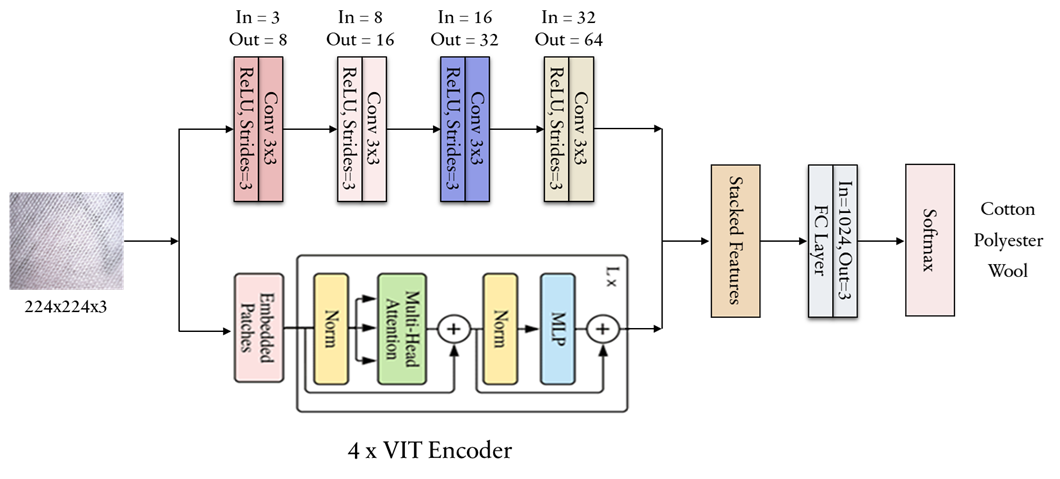
\includegraphics[width=0.95\textwidth]{images/ModelDiagram.png}
    \caption{The proposed hybrid CNN–ViT architecture for fabric classification.}
    \label{fig:model-architecture}
\end{figure}

\paragraph{Softmax Classification}

To generate the final prediction decision, the output logits are softmaxed, to take the raw scores and convert the raw logits to a probability distribution over the three fabric classes:

\[
\text{Softmax}(z_i) = \frac{e^{z_i}}{\sum_{j=1}^{3} e^{z_j}}, \quad \text{for } i = 1,2,3
\]

This is to ensure probabilities are positive, and their sum is 1. The highest probability is selected as the final predicted label. Softmax is the correct choice in multi-class tasks and is a strong performer, especially when used together with cross-entropy loss during training~\cite{bishop2006pattern, goodfellow2016deep}.